%%%%%%%%%%%%%%%%%%%%%%%%%%%%%%%%%%%%%%%%

\begin{frame}
\frametitle{Unbiased means ``Right on Average''}

\begin{block}{Bias of an Estimator}
Let $\widehat{\theta}_n$ be a sample estimator of a population parameter $\theta_0$. The \emph{bias} of $\widehat{\theta}_n$ is $E[\widehat{\theta}_n] - \theta_0$.
\end{block}

\begin{block}{Unbiased Estimator}
A sample estimator $\widehat{\theta}_n$ of a population parameter $\theta_0$ is called \emph{unbiased} if $E[\widehat{\theta}_n]= \theta_0$
\end{block}

\end{frame}


%%%%%%%%%%%%%%%%%%%%%%%%%%%%%%%%%%%%%%%%

\begin{frame}
\frametitle{Why $(n-1)$ for sample variance?}
\alert{We will show that having $n-1$ in the denominator ensures:}
$$E[S^2] =E\left[ \frac{1}{n-1} \sum_{i=1}^n \left(X_i - \bar{X}\right)^2\right] = \sigma^2$$
\alert{under random sampling.}
\end{frame}


%%%%%%%%%%%%%%%%%%%%%%%%%%%%%%%%%%%%%%%%

\begin{frame}
\frametitle{Why $(n-1)$ for sample variance?}
\begin{block}{Step \# 1 -- Tedious but straightforward algebra gives:}
	$$\sum_{i=1}^n \left(X_i - \bar{X}\right)^2 = \left[  \sum_{i=1}^n \left(X_i - \mu\right)^2\right] - n(\bar{X}-\mu)^2$$
\end{block}
\alert{You are not responsible for proving Step \#1 on an exam.}

\end{frame}
%%%%%%%%%%%%%%%%%%%%%%%%%%%%%%%%%%%%%%%%
\begin{frame}
\scriptsize
\begin{eqnarray*}
	\sum_{i=1}^n \left(X_i - \bar{X}\right)^2 &=& \sum_{i=1}^n \left(X_i - \mu + \mu - \bar{X}\right)^2 = \sum_{i=1}^n \left[(X_i -\mu) - (\bar{X} - \mu)\right]^2\\
		&=&\sum_{i=1}^n \left[(X_i -\mu)^2 - 2(X_i -\mu)(\bar{X} - \mu) + (\bar{X} - \mu)^2\right]\\
		&=&\sum_{i=1}^n (X_i -\mu)^2 - \sum_{i=1}^n 2(X_i -\mu)(\bar{X} - \mu) + \sum_{i=1}^n (\bar{X} - \mu)^2\\
		&=& \left[  \sum_{i=1}^n \left(X_i - \mu\right)^2\right]   - 2(\bar{X} - \mu) \sum_{i=1}^n (X_i -\mu)+n(\bar{X} - \mu)^2\\
				&=& \left[  \sum_{i=1}^n \left(X_i - \mu\right)^2\right]   - 2(\bar{X} - \mu) \left( \sum_{i=1}^n X_i- \sum_{i=1}^n \mu \right)+n(\bar{X} - \mu)^2\\
				&=& \left[  \sum_{i=1}^n \left(X_i - \mu\right)^2\right]   - 2(\bar{X} - \mu)(n\bar{X}-n\mu)+n(\bar{X} - \mu)^2\\
				&=&\left[  \sum_{i=1}^n \left(X_i - \mu\right)^2\right]   - 2n(\bar{X} - \mu)^2+n(\bar{X} - \mu)^2\\
				&=&\left[  \sum_{i=1}^n \left(X_i - \mu\right)^2\right]   - n(\bar{X} - \mu)^2
\end{eqnarray*}
\end{frame}

%%%%%%%%%%%%%%%%%%%%%%%%%%%%%%%%%%%%%%%%

\begin{frame}
\frametitle{Why $(n-1)$ for sample variance?}
\begin{block}{Step \# 2 -- Take Expectations of Step \# 1:}
	\begin{eqnarray*}
		E\left[\sum_{i=1}^n \left(X_i - \bar{X}\right)^2\right] &=& E\left[\left\{  \sum_{i=1}^n \left(X_i - \mu\right)^2\right\} - n(\bar{X}-\mu)^2\right]\\
			&=&\pause E\left[ \sum_{i=1}^n \left(X_i - \mu\right)^2\right] -E\left[ n(\bar{X}-\mu)^2\right]\\
			&=&\pause  \sum_{i=1}^n E\left[\left(X_i - \mu\right)^2\right] -n\;E\left[ (\bar{X}-\mu)^2\right]\\
	\end{eqnarray*}
\end{block}
\alert{Where we have used the linearity of expectation.}
\end{frame}
%%%%%%%%%%%%%%%%%%%%%%%%%%%%%%%%%%%%%%%%


\begin{frame}
\frametitle{Why $(n-1)$ for sample variance?}
\begin{block}{Step \# 3 -- Use assumption of random sampling:}
\alert{$X_1, \hdots, X_n \sim \mbox{ iid}$ with mean $\mu$ and variance $\sigma^2$}
	\begin{eqnarray*}
		E\left[\sum_{i=1}^n \left(X_i - \bar{X}\right)^2\right] &=&  \sum_{i=1}^n E\left[\left(X_i - \mu\right)^2\right] -n\;E\left[ (\bar{X}-\mu)^2\right]\\
		&=&  \pause \sum_{i=1}^n Var(X_i) -n\;E\left[ (\bar{X}-E[\bar{X}])^2\right]\\
		&=& \pause   \sum_{i=1}^n Var(X_i) -n\;Var(\bar{X})= n\sigma^2 - \sigma^2\\
		&=& \pause (n-1)\sigma^2
	\end{eqnarray*}
\end{block}
\alert{Since we showed earlier today that  $E[\bar{X}]=\mu$ and $Var(\bar{X})=\sigma^2/n$ under this random sampling assumption.}
\end{frame}
%%%%%%%%%%%%%%%%%%%%%%%%%%%%%%%%%%%%%%%%

\begin{frame}
\frametitle{Why $(n-1)$ for sample variance?}
\begin{block}{Finally -- Divide Step \# 3 by $(n-1)$:}
	\begin{eqnarray*}
		E[S^2] &=& E\left[\frac{1}{n-1}\sum_{i=1}^n \left(X_i - \bar{X}\right)^2\right]= \frac{(n-1)\sigma^2}{n-1} = \sigma^2
	\end{eqnarray*}
\end{block}
\alert{Hence, having $(n-1)$ in the denominator ensures that the sample variance is ``correct on average,'' that is \emph{unbiased}.}
\end{frame}
%%%%%%%%%%%%%%%%%%%%%%%%%%%%%%%%%%%%%%%%
\begin{frame}
\frametitle{A Different Estimator of the Population Variance}

$$\widehat{\sigma}^2 = \frac{1}{n}\sum_{i=1}^n \left(X_i - \bar{X}\right)^2$$
\pause
\begin{eqnarray*}
E[\widehat{\sigma}^2 ] = E\left[\frac{1}{n}\sum_{i=1}^n \left(X_i - \bar{X}\right)^2  \right]= \frac{1}{n} E\left[\sum_{i=1}^n \left(X_i - \bar{X}\right)^2\right] = \pause \frac{(n-1)\sigma^2}{n} 
\end{eqnarray*}

\begin{block}{Bias of $\widehat{\sigma}^2$}
\vspace{0.75em}
$\displaystyle E[\widehat{\sigma}^2 ] - \sigma^2 = \pause \frac{(n-1)\sigma^2}{n}  - \sigma^2 = \frac{(n-1)\sigma^2}{n}  - \frac{n\sigma^2}{n} = -\sigma^2/n$
\end{block}
\end{frame}
%%%%%%%%%%%%%%%%%%%%%%%%%%%%%%%%%%%%%%%%

\begin{frame}
\frametitle{How Large is the Average Family? \hfill
\includegraphics[scale = 0.05]{./images/clicker}}

\Large How many brothers and sisters are in your family, including yourself?

\end{frame}

%%%%%%%%%%%%%%%%%%%%%%%%%%%%%%%%%%%%%%%%
\begin{frame}
\Large
\alert{The average number of children per family was about 2.0 twenty years ago.}
\end{frame}
%%%%%%%%%%%%%%%%%%%%%%%%%%%%%%%%%%%%%%%%
\begin{frame}
\frametitle{What's Going On Here?}
\pause
Biased Sample!
\begin{itemize}
 	\item  Zero children $\Rightarrow$ didn't send any to college
 	\item Sampling by \emph{children} so large families \alert{oversampled}
\end{itemize}


\end{frame}
%%%%%%%%%%%%%%%%%%%%%%%%%%%%%%%%%%%%%%%%

\begin{frame}[fragile]



\frametitle{Candy Weighing: 49 Estimates, Each With $n=5$}

\begin{columns} 
\begin{column}[c]{5cm} 
\small

$$\widehat{\theta} = 20 \times (X_1 + \hdots + X_5)$$

\small
 %FIRST COLUMN HERE
   \begin{tabular}{lr}
   \hline \hline
   \multicolumn{2}{l}{Summary of Sampling Dist.} \\
   \hline
   Overestimates& 45\\
   Exactly Correct& 0\\
   Underestimates& 4\\
   \hline
   $E[\hat{\theta}]$& 1164 grams\\
   SD$(\widehat{\theta})$& 189 grams\\
   \hline
   \end{tabular}
   
  \vspace{1em}
  Actual Mass:  $\theta_0 =$932 grams
\end{column} 
\begin{column}[c]{5cm} 

 %SECOND COLUMN HERE 
\begin{figure}
\centering
\begin{knitrout}
\definecolor{shadecolor}{rgb}{0.969, 0.969, 0.969}\color{fgcolor}

{\centering \includegraphics[width=\maxwidth]{figure/unnamed-chunk-2-1} 

}



\end{knitrout}


\end{figure}

\end{column} 
\end{columns} 


\end{frame}

%%%%%%%%%%%%%%%%%%%%%%%%%%%%%%%%%%%%%%%%
\begin{frame}
\frametitle{What was in the bag?}

100 Candies Total:
\begin{itemize}
	\item 20 Fun Size Snickers Bars (large) 
	\item 30 Reese's Miniatures (medium) 
	\item 50 Tootsie Roll ``Midgees'' (small)
\end{itemize}
\begin{block}{So What Happened?}
	\pause Not a random sample! The Snickers bars were \emph{oversampled}.
\end{block}
\begin{block}{Could we have avoided this? How?}

\end{block}
\end{frame}

%%%%%%%%%%%%%%%%%%%%%%%%%%%%%%%%%%%%%%%%
\begin{frame}
\frametitle{
\includegraphics[scale = 0.05]{./images/clicker}}
Let $X_1, X_2, \hdots X_n \sim iid$ mean $\mu$, variance $\sigma^2$ and define $\bar{X}_n = \frac{1}{n}\sum_{i=1}^n X_i$. True or False:

\vspace{1em}
\begin{quotation}
$\bar{X}_n$ is an unbiased estimator of $\mu$
\end{quotation}

\begin{enumerate}[(a)]
\item True
\item False
\end{enumerate}
\pause

\alert{TRUE!}

\end{frame}

%%%%%%%%%%%%%%%%%%%%%%%%%%%%%%%%%%%%%%%%
\begin{frame}
\frametitle{
\includegraphics[scale = 0.05]{./images/clicker}}
Let $X_1, X_2, \hdots X_n \sim iid$ mean $\mu$, variance $\sigma^2$. True or False:

\vspace{1em}
\begin{quotation}
$X_1$ is an unbiased estimator of $\mu$
\end{quotation}

\begin{enumerate}[(a)]
\item True
\item False
\end{enumerate}

\pause \alert{TRUE!}
\end{frame}
%%%%%%%%%%%%%%%%%%%%%%%%%%%%%%%%%%%%%%%%
\begin{frame}
\frametitle{How to choose between two unbiased estimators?}

Suppose $X_1, X_2, \hdots X_n \sim iid$ with mean $\mu$ and variance $\sigma^2$
\begin{eqnarray*}
E[\bar{X}_n] &=& E\left[\frac{1}{n}\sum_{i=1}^n X_i\right] = \frac{1}{n}\sum_{i=1}^n E[X_i] = \mu\\
E[X_1] &=& \mu\\
\pause
Var(\bar{X}_n) &=& Var\left(\frac{1}{n}\sum_{i=1}^n X_i\right) = \frac{1}{n^2} \sum_{i=1}^n Var(X_i) = \alert{\sigma^2/n}\\
\pause
Var(X_1) &=& \alert{\sigma^2}
\end{eqnarray*}
\end{frame}
%%%%%%%%%%%%%%%%%%%%%%%%%%%%%%%%%%%%%%%%

\begin{frame}
\frametitle{Efficiency - Compare Unbiased Estimators by Variance}
Let $\widehat{\theta}_1$ and $\widehat{\theta}_2$ be unbiased estimators of $\theta_0$. We say that $\widehat{\theta}_1$ is \alert{\emph{more efficient}} than $\widehat{\theta}_2$ if $Var(\widehat{\theta}_1)<Var(\widehat{\theta}_2)$.
\end{frame}

%%%%%%%%%%%%%%%%%%%%%%%%%%%%%%%%%%%%%%%%
\begin{frame}
\frametitle{Mean-Squared Error}
Except in very simple situations, unbiased estimators are hard to come by. In fact, in many interesting applications there is a \alert{\emph{tradeoff}} between \alert{bias} and \alert{variance}:
\begin{itemize}
\item Low bias estimators often have a high variance 
\item Low variance estimators often have high bias
\end{itemize}
\pause
\vspace{1em}
\alert{Mean-Squared Error (MSE):}   Squared Bias plus Variance
$$ MSE(\widehat{\theta}) = \mbox{Bias}(\widehat{\theta})^2 + Var(\widehat{\theta})$$ 

\alert{Root Mean-Squared Error (RMSE):} $\sqrt{\mbox{MSE}}$  

\end{frame}
%%%%%%%%%%%%%%%%%%%%%%%%%%%%%%%%%%%%%%%%
\begin{frame}
\frametitle{Calculate MSE for Candy Experiment \hfill 
\includegraphics[scale = 0.05]{./images/clicker}}


\begin{columns} 

\begin{column}[c]{4cm} 
 %SECOND COLUMN HERE 
\begin{figure}
\begin{knitrout}
\definecolor{shadecolor}{rgb}{0.969, 0.969, 0.969}\color{fgcolor}

{\centering \includegraphics[width=\maxwidth]{figure/unnamed-chunk-3-1} 

}



\end{knitrout}
\end{figure}

\end{column} 

\begin{column}[c]{6cm} 
\small
 %FIRST COLUMN HERE
   \begin{tabular}{lr}
   \hline
   \hline
   $E[\hat{\theta}]$& 1164 grams\\
   $\theta_0$& 932 grams\\
   $SD(\widehat{\theta})$& 189 grams\\
   \hline
   \end{tabular}
\vspace{2em}

\begin{eqnarray*}
	\mbox{Bias} &=& \pause 1164 \mbox{ grams} - 932 \mbox{ grams}\\
		&=& \alert{232 \mbox{ grams}}\\
		\mbox{MSE} &=&\pause  \mbox{Bias}^2 + \mbox{Variance}\\
			&=& (232^2 + 189^2)\mbox{ grams}^2\\
				&=&\pause \ensuremath{8.9545\times 10^{4}} \mbox{ grams}^2\\ \pause
				\mbox{RMSE} &=& \sqrt{\mbox{MSE}} =  299 \mbox{ grams}
\end{eqnarray*}
\end{column} 

\end{columns} 


\end{frame}
%%%%%%%%%%%%%%%%%%%%%%%%%%%%%%%%%%%%%%%%
\begin{frame}
\frametitle{Finite Sample versus Asymptotic Properties of Estimators}

\begin{block}{Finite Sample Properties}
For \alert{\emph{fixed sample size $n$}} what are the properties of the sampling distribution of $\widehat{\theta}_n$? (E.g.\ bias and variance.)
\end{block}
\begin{block}{Asymptotic Properties}
What happens to the sampling distribution of $\widehat{\theta}_n$ \alert{\emph{as the sample size $n$ gets larger and larger?}} (That is, $n\rightarrow \infty$).
\end{block}

\end{frame}
%%%%%%%%%%%%%%%%%%%%%%%%%%%%%%%%%%%%%%%%
\begin{frame}
\frametitle{Why Asymptotics?}

\begin{block}{Law of Large Numbers}
Make precise what we mean by ``bigger samples are better.'' 
\end{block}
\begin{block}{Central Limit Theorem}
As $n\rightarrow \infty$  \emph{\alert{pretty much any}} sampling distribution is well-approximated by a normal random variable!
\end{block}


\end{frame}
%%%%%%%%%%%%%%%%%%%%%%%%%%%%%%%%%%%%%%%%
\begin{frame}
\frametitle{Consistency}

\begin{block}{Consistency}
If an estimator $\widehat{\theta}_n$ (which is a RV) \emph{converges} to $\theta_0$ (a constant) as $n\rightarrow \infty$, we say that \emph{\alert{$\widehat{\theta}_n$ is consistent for $\theta_0$}}.
\end{block}
\vspace{2em}

\begin{alertblock}{What does it mean for a \emph{RV} to converge to a \emph{constant?}}
For this course we'll use \emph{MSE Consistency}:
	$$\lim_{n \rightarrow \infty}\mbox{MSE}(\widehat{\theta}_n) = 0$$
This makes sense since MSE$(\widehat{\theta}_n)$ is a \emph{constant}, so this is just an ordinary limit from calculus.
\end{alertblock}

\end{frame}

%%%%%%%%%%%%%%%%%%%%%%%%%%%%%%%%%%%%%%%%
\begin{frame}
\frametitle{Law of Large Numbers (aka Law of Averages)}
Let $X_1, X_2, \hdots X_n \sim iid$ mean $\mu$, variance $\sigma^2$. Then the sample mean 
	$$\bar{X}_n = \frac{1}{n}\sum_{i=1}^n X_i$$
is consistent for the population mean $\mu$.
\end{frame}

%%%%%%%%%%%%%%%%%%%%%%%%%%%%%%%%%%%%%%%%



\begin{frame}
\frametitle{Law of Large Numbers (aka Law of Averages)}
Let $X_1, X_2, \hdots X_n \sim iid$ mean $\mu$, variance $\sigma^2$. 
	\begin{eqnarray*}
			E[\bar{X}_n] &=&  E \left[\frac{1}{n}\sum_{i=1}^n X_i\right] = \mu\\\\ 
      Var(\bar{X}_n) &=& Var\left(\frac{1}{n}\sum_{i=1}^n X_i  \right) = \sigma^2/n\\\\ \pause
			\mbox{MSE}(\bar{X}_n) &=& \mbox{Bias}(\bar{X}_n)^2 + Var(\bar{X}_n)\\\pause
				&=& \left(E[\bar{X_n}] - \mu\right)^2 + Var(\bar{X}_n)\\ \pause
				&=& 0 + \sigma^2/n\\ 
				&\rightarrow& 0
	\end{eqnarray*}
	\alert{Hence $\bar{X}_n$ is consistent for $\mu$}
\end{frame}

%%%%%%%%%%%%%%%%%%%%%%%%%%%%%%%%%%%%%%%%
\begin{frame}
\frametitle{Important! }

An estimator \emph{can} be biased but still consistent, as long as the bias disappears as $n \rightarrow \infty$
$$\widehat{\sigma}^2 = \frac{1}{n}\sum_{i=1}^n \left(X_i - \bar{X}\right)^2$$


\begin{block}{Bias of $\widehat{\sigma}^2$}
\vspace{0.75em}
$\displaystyle E[\widehat{\sigma}^2 ] - \sigma^2 = \pause \frac{(n-1)\sigma^2}{n}  - \sigma^2 =  \pause -\sigma^2/n \pause \rightarrow 0$
\end{block}


\end{frame}

%%%%%%%%%%%%%%%%%%%%%%%%%%%%%%%%%%%%%%%%



\begin{frame}
\frametitle{
\includegraphics[scale = 0.05]{./images/clicker}}
Suppose $X_1, X_2, \hdots, X_n \sim \mbox{iid } N(\mu,\sigma^2)$. What is the sampling distribution of $\bar{X}_n$?

\begin{enumerate}[(a)]
\item $N(0,1)$
\item $N(\mu, \sigma^2/n)$
\item $N(\mu, \sigma^2)$
\item $N(\mu/n, \sigma^2/n)$
\item $N(n\mu, n\sigma^2)$
\end{enumerate}

\end{frame}
%%%%%%%%%%%%%%%%%%%%%%%%%%%%%%%%%%%%%%%%

\begin{frame}
\huge\begin{center} But still, how can something random converge to something constant? \end{center}
\end{frame}

%%%%%%%%%%%%%%%%%%%%%%%%%%%%%%%%%%%%%%%%
\begin{frame}
\frametitle{Sampling Distribution of $\bar{X}_n$ Collapses to $\mu$}
Look at an example where we can directly calculate not only the mean and variance of the sampling distribution of $\bar{X}_n$, but the \emph{sampling distribution itself}:

\vspace{1em}
$$\alert{X_1, X_2, \hdots, X_n \sim \mbox{iid } N(\mu,\sigma^2) \Rightarrow \bar{X}_n \sim N(\mu, \sigma^2/n)}$$


\end{frame}




%%%%%%%%%%%%%%%%%%%%%%%%%%%%%%%%%%%%%%%%


\begin{frame}
\frametitle{Sampling Distribution of $\bar{X}_n$ Collapses to $\mu$}
\alert{$X_1, X_2, \hdots, X_n \sim \mbox{iid } N(\mu,\sigma^2 \Rightarrow \bar{X}_n \sim N(\mu, \sigma^2/n)$.} \\
\begin{figure}
\centering
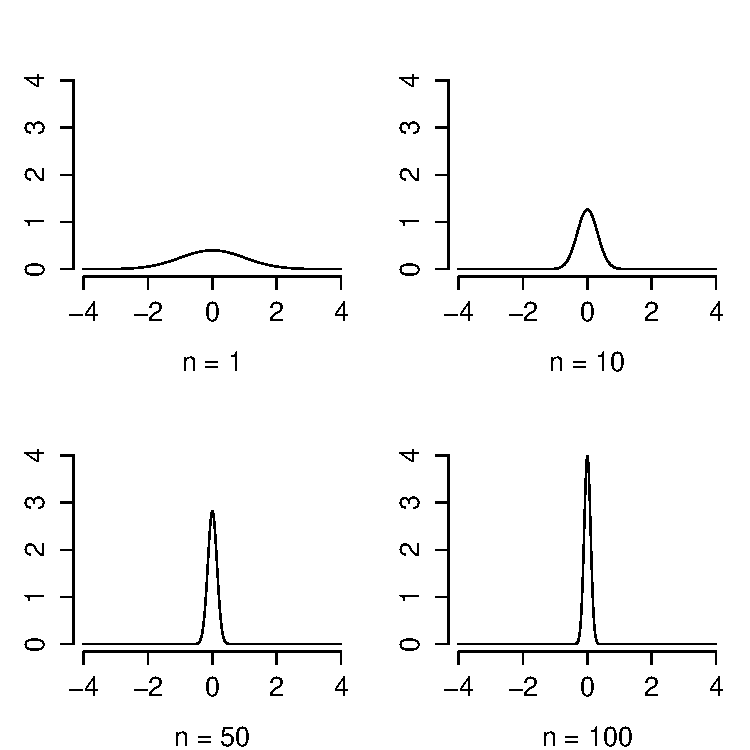
\includegraphics[scale = 0.5]{./images/normal_LLN_dist}
\caption{Sampling Distributions for $\bar{X}_n$ where $X_i \sim \mbox{iid } N(0,1)$}
\end{figure}

\end{frame}




%%%%%%%%%%%%%%%%%%%%%%%%%%%%%%%%%%%%%%%%


\begin{frame}
\frametitle{Another Visualization: Keep Adding Observations}
\begin{columns} 
\begin{column}[c]{8cm} 
 %FIRST COLUMN HERE 
\begin{figure}
\centering
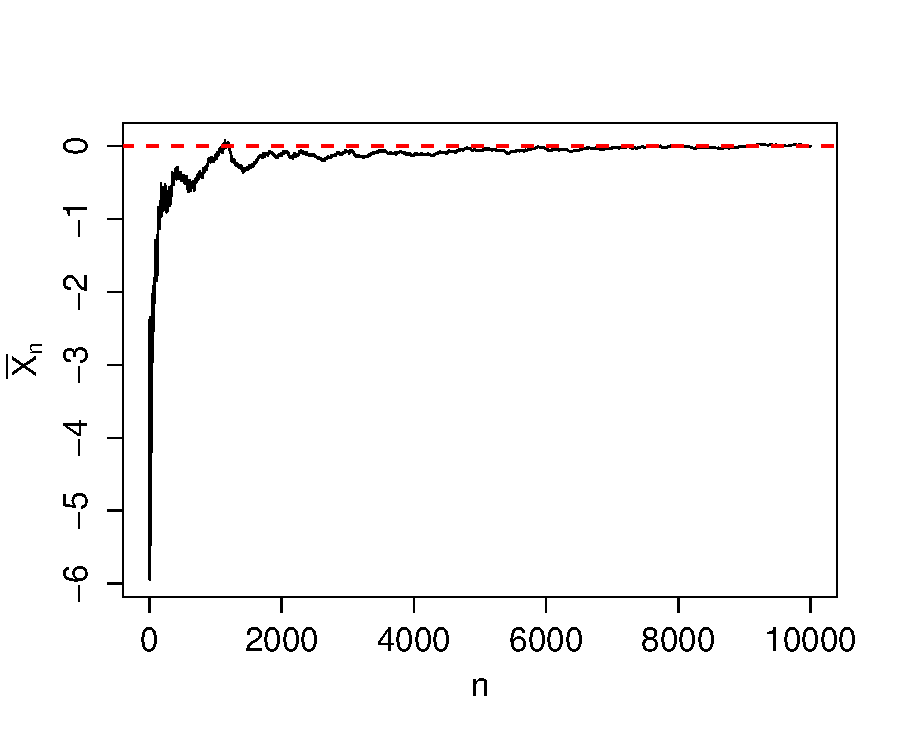
\includegraphics[scale = 0.5]{./images/WLLN}
\caption{Running sample means: $X_i \sim \mbox{iid } N(0, 100)$}
\end{figure}
\end{column} 
\begin{column}[c]{3cm} 

 %SECOND COLUMN HERE 
\footnotesize
\begin{table}
\begin{tabular}{|rr|}
\hline
$n$&$\bar{X}_n$\\
\hline
1 &-2.69\\
2 &-3.18\\
3 &-5.94\\
4 &-4.27\\
5 &-2.62\\
10& -2.89\\
20& -5.33\\
50 &-2.94\\
100& -1.58\\
500 &-0.45\\
1000& -0.13\\
5000& -0.05\\
10000&  0.00\\
\hline
\end{tabular}
\end{table}

\end{column} 
\end{columns} 


\end{frame}
%%%%%%%%%%%%%%%%%%%%%%%%%%%%%%%%%%%%%%%%
